\documentclass[twocolumn]{article}
\usepackage[top = 1in, bottom = 1in, left = .75in, right = .75in]{geometry} % Cusomize your margins and page size
\usepackage{fancyhdr} %% Fancy header package
%% =-=-=-=-=-=-=-=-=-=-=-=-=-
% Fancy Header parameters
%% =-=-=-=-=-=-=-=-=-=-=-=-=-
\pagestyle{fancy} % Change all pages to use the fancy header style.
\cfoot{} % Clear {c}enter {foot}er
\lfoot{\thepage} % Display `\thepage' on the {l}eft {foot}er
\rhead{Beginning \LaTeX} % Place a running {r}ight {head}er

%% =-=-=-=-=-=-=-=-=-=-=-=-=-
% Organize
%% =-=-=-=-=-=-=-=-=-=-=-=-=-
\usepackage{booktabs, tabularx} %% Tables
\usepackage{hyperref} %% Links through your paper and to URLs

\usepackage{mathtools, amssymb, amsthm} %% The AMS series!
\usepackage{graphicx, float} %% For importing images

\begin{document}
Now that we can generate a basic TeX file, we can begin to be picky. The main power of LaTeX is the customization. But instead of making everything on your own, you can use pre-existing customizations. These come in \verb|packages|, sometimes refered to as \verb|style| files, or .sty.

\section{Packages}\label{sec:packages}
Packages will allow you deep customizations for your document. The reserved space for declaring which packages are being used is between \verb|\documentclass{}| and \verb|\begin{document}|.\footnote{The space before \texttt{\textbackslash begin\{document\}} is the \texttt{preamble}}

The LaTeX compiler will read through these sequentially to be able to use the customizations provided. In some rare cases, the order of packages will matter. To \verb|load| or \verb|import| a package, we can write \verb|\usepackage{|$\bullet$\verb|}|.

\subsection{Packages with options and parameters}
To allow for this customization, packages will have many options and specifications that the user can set.

For example, the \verb|geometry| package provides control over the margins for your document and also the page size. These have default values set by the .cls file, but this package safely overrides those values. These are set by changing \verb|options| for the package. This introduces \textit{optional} arguments, which are grouped within square braces [] as the TeX norm. For example, to use the \verb|geometry| package, we can set our margins by setting the optional arguments: \verb|top = 1in| changes the top margin to be .75 inches, etc. Another possible option is to use \verb|margin = | for all margins. Other commands and even your document class can have optional arguments as well.\footnote{See \texttt{twocolumn} option in the \texttt{documentclass}}

The \verb|fancyhdr| package gives full control over headers and footers. This package allows you to define \verb|parameters| that the package will use throughout your document. These parameters must be set after you load the package, but before you begin your document. 
\href{https://www.overleaf.com/learn/latex/Headers_and_footers#LaTeX_document_classes}{See this link if you want a thorough guide.}\footnote{These hyperlinks are made possible by the \texttt{hyperref} package. Which is also useful for in document links to theorems/definitions/etc.}

\subsection{\texttt{ams} series of packages}
These packages contain everything you need for math.
\begin{itemize}
    \item \texttt{mathtools} - An extension of \verb|amsmath| (which it also loads for free) which introduces some bug fixes, extra settings, and more! It will essentially contain anything you need for typesetting math and more. For a better documentation, see \href{https://www.overleaf.com/learn/latex/Articles/Mathtools_-_for_beautiful_math}{this link.}
    \item \texttt{amssymb} - Additional math symbols. An extension of \verb|amsfont|, so this is a superset package.
    \item \texttt{amsthm} - Helps you define theorem-like structure. Most importantly, it provides the \verb|\newtheorem| command and the \verb|proof| environment which autocompletes with a QED symbol at the end.
\end{itemize}
There are some ams document classes where these are automatically loaded, but for our use cases, it is a bit of a moot point.

\subsubsection{Alignment}
One benefit of loading \verb|mathtools| is the introduction to many powerful alignment environments.

First we can consider the \verb|align| and \verb|align*| environments, which are used to show mutlistep solutions to equations.
\begin{verbatim}
\begin{align}
    2x+4 &= 6\\
    2x &= 2\\
    x &= 1
\end{align}  
\end{verbatim}
\noindent Will display as:
\begin{align}
    2x+4 &= 6\\
    2x &= 2\\
    x &= 1
\end{align}

Some things to note are that the \&'s define the alignment. When using alignment LaTeX will use \& symbols for horizontal spacing. For \verb|align| and \verb|align*|, LaTeX will attempt to match \&'s vertically. Another visualization is that these environments define two columns. Text in the left column is right justified and text in the right column is left justified and columns are separated at the \& symbol.

Another key part here is that we use \textbackslash\textbackslash to break lines. This is required in math mode for line breaks in many \verb|mathtools| environments for TeX to better sparse white spaces.

The \verb|align*| environment removes the labeling of the lines. But you can manually add labels by using the \verb|tag| command on a line. For example,
\begin{verbatim}
\begin{align*}
    x^2  - 1 &= 0\\
    (x+1)(x-1)&=0\tag{Diff of Squares}\\
    x &= \pm 1
\end{align*}
\end{verbatim}
\begin{align*}
    x^2  - 1 &= 0\\
    (x+1)(x-1)&=0\tag{Diff of Squares}\\
    x &= \pm 1
\end{align*}

Another collection of environments introduced in the \verb|mathtools| package are the \verb|matrix| environments. Within this collection we have:\begin{itemize}
    \item \verb|matrix| - Generates an un-bordered array within math mode
    \item \verb|pmatrix| - Generates a \textbf{p}arenthesesed array within math mode
    \item \verb|bmatrix| - Square \textbf{b}racketed
    \item \verb|Bmatrix| - Curly \textbf{B}racketed
    \item \verb|vmatrix| - \textbf{v}erticals; determinant notation
    \item \verb|Vmatrix| - Double \textbf{V}erticals; norm notation
\end{itemize}
For example:
\begin{verbatim}
\[\begin{pmatrix}
    4 & 6 & 3\\
      & 3 & x_4
\end{pmatrix}\]
\end{verbatim}

will generate the following matrix in a \verb|displaymath| environment
\[\begin{pmatrix}
    4 & 6 & 3\\
      & 3 & x_4
\end{pmatrix}\]
Similarly to the \verb|align| environment, \&'s are used to denote the end of a column/beginning of the next. We can leave columns empty if we want as well. The \verb|matrix| environments are clean as they will automatically parse how many columns the matrix will have. In other environments, we will have to manually define this parameter.

Another alignment environment is the \verb|cases| environment.
\begin{verbatim}
\[H_n(T^2) = \begin{cases}
    \mathbb{Z}   & n = 0, 2\\
    \mathbb{Z}^2 & n = 1\\
    0            & \text{else}
\end{cases}\]
\end{verbatim}
\[H_n(T^2) = \begin{cases}
    \mathbb{Z}   & n = 0, 2\\
    \mathbb{Z}^2 & n = 1\\
    0            & \text{else}
\end{cases}\]

\subsection{Basic Tables}
To generate a table, we use the \verb|tabular| environment, as the \verb|table| environment is reserved as a keyword for a float environment. The \verb|tabular| environment has a required parameter which defines the number of columns, their justification, and how to separate them. Within the \verb|tabular|, some commands will be scaled to the width of the table, such as \verb|\hline|.
\begin{verbatim}
\begin{tabular}{c|l||r}
    {c}entered & {l}eft just. & {r}ight \\\hline
    x & y & z\\
    1 & 2 & 3
\end{tabular}
\end{verbatim}

\begin{tabular}{c|l||r}
    {c}entered & {l}eft just. & {r}ight \\\hline
    x & y & z\\
    1 & 2 & 3
\end{tabular}

The parameter \begin{verbatim}|{c|l||r}|\end{verbatim} tells TeX that the first column will be centered, separated from the second column by a single vertical line, which is left justified and is separated from the final right justified column by two vertical lines.

For an easier way of typesetting tables, we can use a \href{https://www.tablesgenerator.com/}{table generator}. This specific example lets us choose which table customization package to use.\footnote{The author prefers \texttt{booktabs}} Then you can simply copy and paste the table into a TeX project.

\subsection{How to find packages, parameters, options}
While most math symbols are in the \texttt{ams} packages, sometimes you need something niche. A safe bet is to Google for your symbol, but another nice option is:
\begin{itemize}
    \item \href{https://detexify.kirelabs.org/classify.html}{Detexify is a drawing $\to$ command search site}
\end{itemize}
When using a package, you can often find its documentation on \href{https://ctan.org}{CTAN}, where its developers will provide a full list of commands, options, parameters, and example usages.

\section{Text Formatting}
Regular text formatting offered by other word processors are offered in LaTeX via commands.\begin{itemize}
    \item \verb|\textbf{}| - \textbf{bold text}, used outside of math mode, \verb|ctrl + b| Overleaf hotkey
    \item \verb|\mathbb{}| - blackboard bold, used inside math mode. ex: $\mathbb{R,C,Q}$
    \item \verb|\textit{}| - \textit{italicized}, used outside of math mode, \verb|ctrl + i| Overleaf hotkey
    \item \verb|\emph{}| - \emph{emphasized} words. Not always italicized, can change depending on package/document class, or by your own modification
    \item \verb|\mathcal{}| - math cursive, used inside math mode. ex: $\mathcal{T, C,M}$
    \item \verb|\underline{}| - underlined text
    \item \verb|\underbrace{}_{}| - $\underbrace{\text{Underbraces inside math mode}}_{\text{with an option for text below}}$
    \item \verb|\overbrace{}^{}| - similarly
\end{itemize}
There are also commands for changing font size. font, etc. But often you will work in a standard font size, and use Computer Modern Serif, which is the standard LaTeX font. If you are interested in changing anything, see \href{https://www.overleaf.com/learn/latex/Font_sizes%2C_families%2C_and_styles}{this page}.

\section{Figures, tables, and labels}
Before we insert images/figures/tables, we first introduce \verb|float environments|. These are environments that create a chunk of space whose placement on the page can be modified. Often, the default behavior is all you need, but sometimes you want to be more precise. The three most commonly used float environments are \verb|figure| and \verb|table|. There are also various packages that contain an \verb|algorithm| environment for code/pseudocode, such as \verb|algorithms2e| or \verb|algpseudocode|. The general setup for these would be:
\begin{verbatim}
\begin{floatEnv}[Float Parameter]
    \label{envLabel:ObjectLabel}
    *Insert figure/table/algorithm*
    \caption[]{A caption for the image.}
\end{floatEnv}
\end{verbatim}\setcounter{figure}{0}
The float parameter can be empty for LaTeX to choose where to place the figure, or you can use one of the following:
\begin{itemize}
    \item \verb|h| - Place the environment \textit{approximately} here
    \item \verb|H| - Place the environment \textit{exactly} here, requires the \verb|float| package
    \item \verb|t| - Place the environment at the top of the page
    \item \verb|b| - Place the environment at the bottom of the page
    \item \verb|p| - Place the environment on a page reserved for float environments 
\end{itemize}
For more details and more precise control options, see \href{https://en.wikibooks.org/wiki/LaTeX/Floats,_Figures_and_Captions}{this page.}

As a running example, we have the following below. Where the line breaks during the \verb|includegraphics| and \verb|\caption| command are for text width considerations.
\begin{verbatim}
\begin{figure}[H]
    \label{fig:GMA_Logo}
    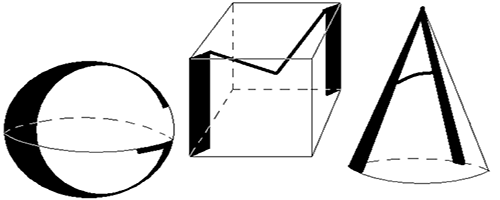
\includegraphics[width = .5\textwidth]
        {Figures/GMA-logo.png}
    \caption[Short caption]
        {Longer display caption.}
\end{figure}
\end{verbatim}

\begin{figure}[H]
    \label{fig:GMA_Logo}
    \centering
    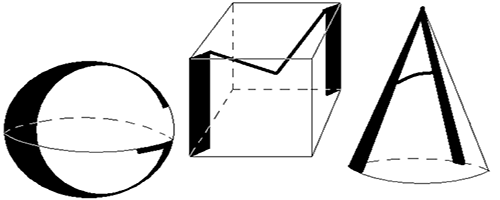
\includegraphics[width = .25\textwidth]{Figures/GMA-logo.png}
    \caption[Short caption]{Longer display caption.}
\end{figure}

Here, we use \verb|[H]| as the placement argument to force the image to appear below the displayed \verb|verbatim| text. We assign the figure a \verb|label|, which we can use \verb|hyperref| to create a link to the figure. Academic papers require references to each figure/table included in a paper. For example: \verb|``See Figure~\ref{fig:GMA_Logo} for an example| \verb|of how to include a figure."| generates the following: ``See Figure~\ref{fig:GMA_Logo} for an example of how to include a figure. We can place \verb|labels| anywhere we want to point towards. Generally, you want labels for all figures, (sub)sections, etc. For example, if you want to review how to load packages, see Section~\ref{sec:packages}. LaTeX by default enumerates various environments. This allows it to properly track and display values. For example, we can point to Section~\ref{sec:Errors} which will properly display the correct section number without labeling all the sections.

Generally, labels are formatted in a method for easy searches. For example, figures can be labeled \verb|fig:FigureLabel|, the \verb|fig| prefix denoting it to be a figure, \verb|FigureLabel| as a unique identifier, and \verb|:| is used to distinguish the two. This is for easy reference searching for larger projects and for understanding during collaboration.

Other examples of automatic labels and references are \verb|footnotes|, which are easy enough to apply.\verb|\footnote{This will be automatically| \verb|generated and placed below.}|\footnote{This will be automatically generated and placed below.} Bibliographies will similarly be automatically labeled and sorted for quick referencing. We will cover bibliographies when talking about larger projects.
\section{Error Handling}\label{sec:Errors}
When we get compilation errors, the best way to remedy them is to look for keywords. Throughout these pages, I have tried to define certain keywords for easier translation of errors into English. If you have an error you cannot parse, a search engine is your best friend. But as a list of common errors in no particular order:
\begin{itemize}
    \item Missing math mode
    \item Missing matching curly braces
    \item incorrect commands
    \item Too many/few alignment indicators
\end{itemize}
There are also warnings, which can often be ignored. For example, this document has a lot of the following warnings, and I don't have the energy to fix them.
\begin{itemize}
    \item `hbox full': You've exceeded the text width by force somehow. A figure, a forced grouping, etc. For example,

    \verb|This is a really long line of text that and there will be a warning|
\end{itemize}
\end{document}